\subsection{Уравнение движения материальной точки. Третий закон Ньютона. Силы трения. Сила упругости}

\begin{definition}
    Третий закон Ньютона (закон взаимодействия тел).

    Сила действия равна силе противодействия.

    Силы взаимодействия двух материальных точек равны по величине, противоположно направлены и действуют вдоль прямой, соединяющей эти материальные точки.
\end{definition}

$$\vec F_1=-\vec F_2$$

\begin{definition}
    Сила упругости (сила реакции опоры) — сила, направленная против деформации тела, по модулю равная силе, деформирующей это тело.
\end{definition}

Виды деформации:
\begin{itemize}
    \item Упругая: тело принимает первоначальную форму и размеры после того, как сила перестала действовать.
    \item Пластическая: тело сохраняет те формы и размеры, которое приобрело под действием силы.
\end{itemize}

Деформация обусловлена электрическим воздействием между атомами. Если атомы удалять друг от друга, то между ними возникает сила притяжения 
(между ядром и электронной оболочкой). Если приближать атомы друг к другу, то возникает сила отталкивания (между ядрами)

\begin{definition} Закон Гука \end{definition}

\centering
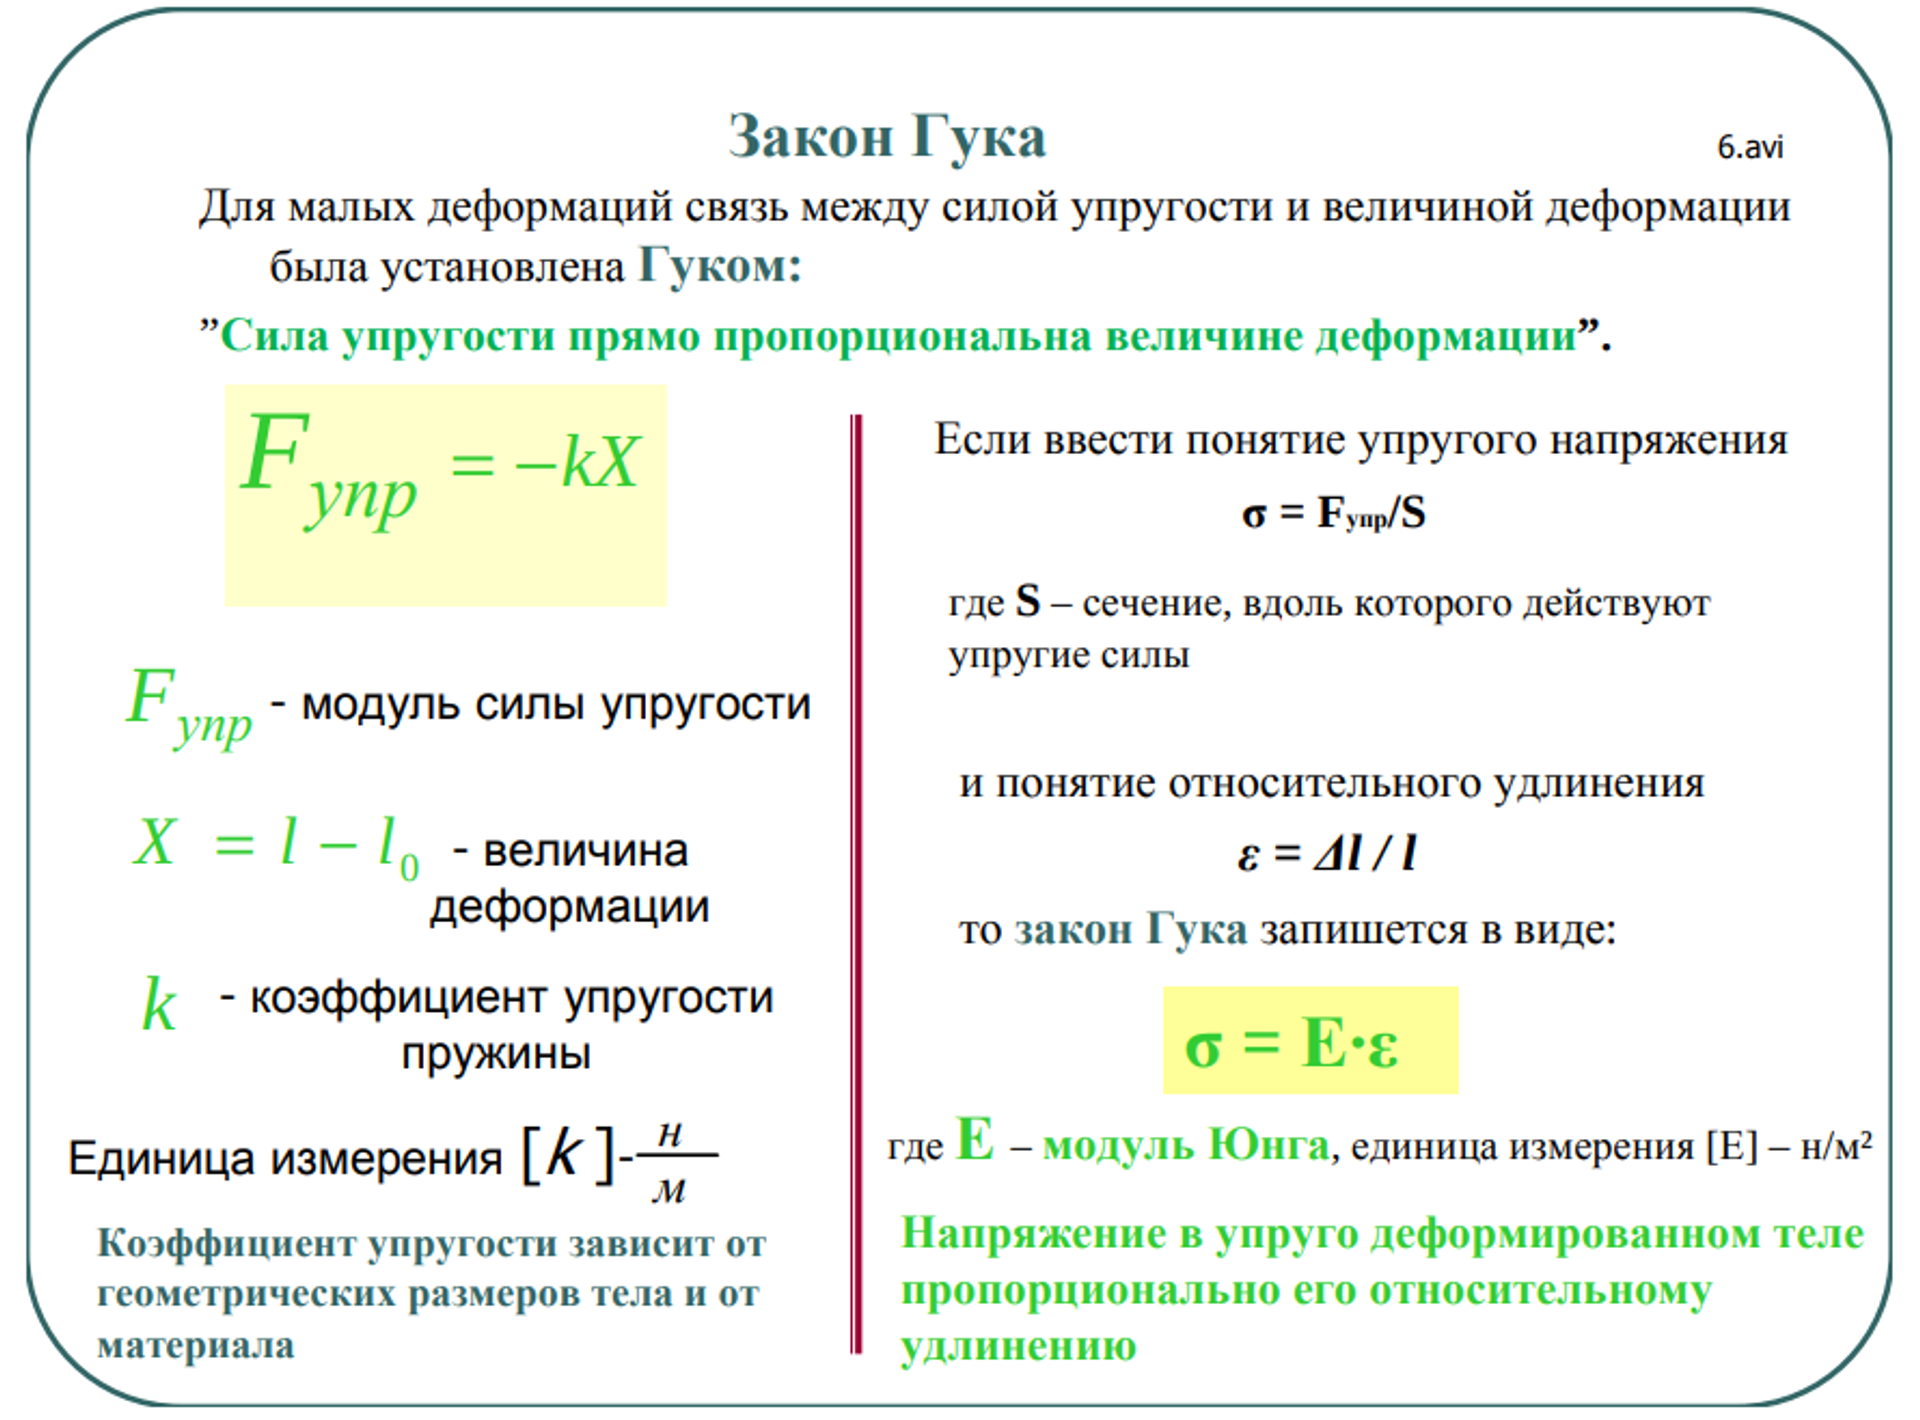
\includegraphics[width=0.7\linewidth]{imgs/q5i1.png}
\centering
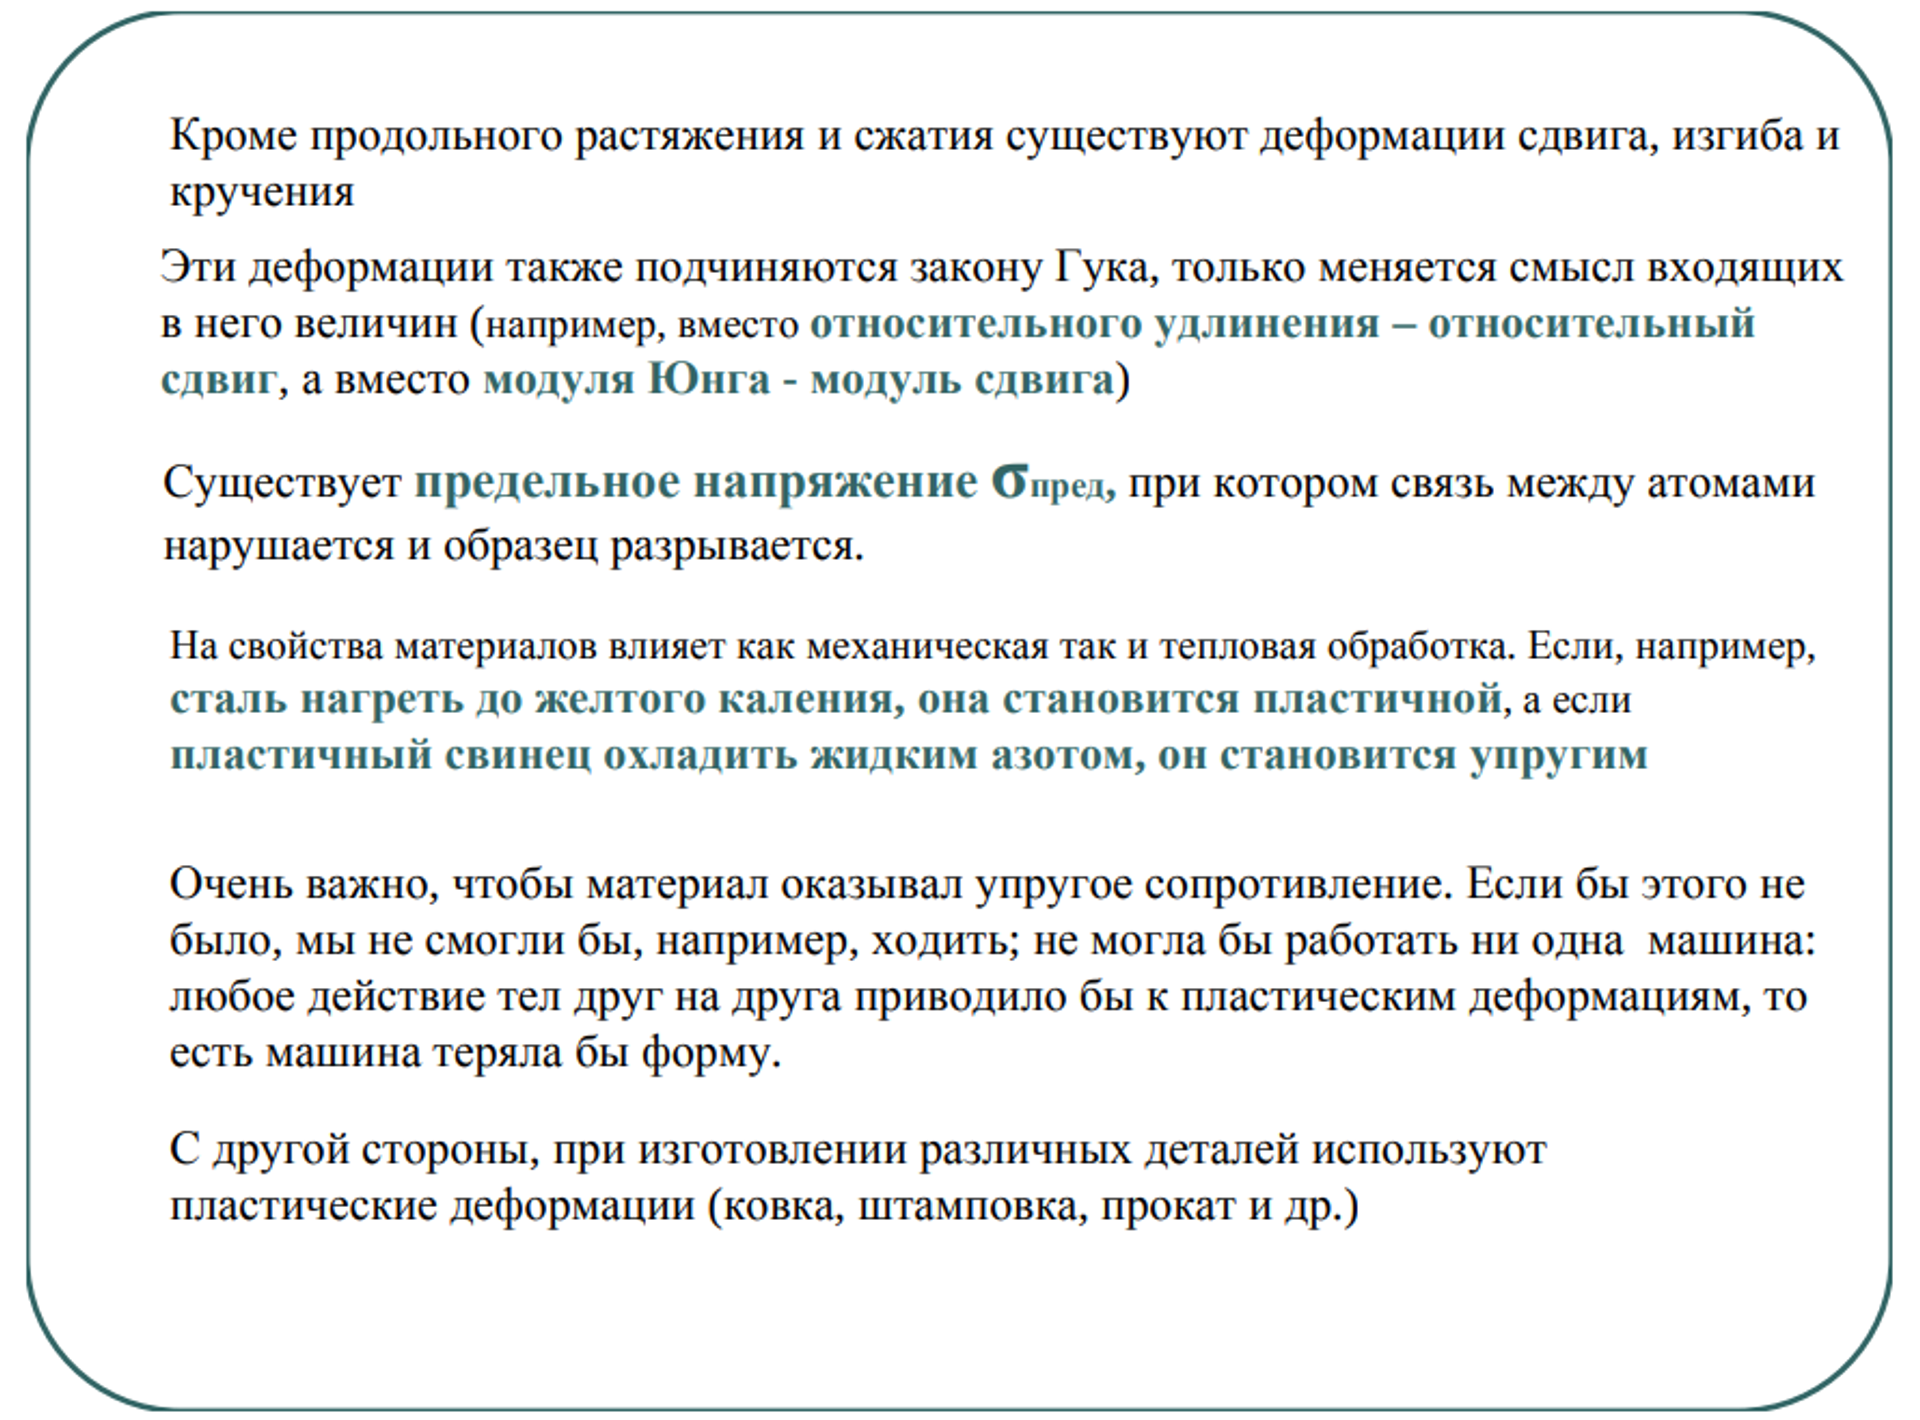
\includegraphics[width=0.7\linewidth]{imgs/q5i2.png}

\begin{definition}
    Силы трения.

    Сила трения возникает при непосредственном соприкосновении двух тел и препятствует движению этих тел.

    Сила трения, подобно силе упругости, является проявлением электрического взаимодействия атомов.
\end{definition}


\begin{enumerate}
    \item Сила трения покоя — сила, возникающая между двумя неподвижными контактирующими телами и препятствующая возникновению относительного движения.
    
    Эту силу необходимо преодолеть для того, чтобы привести два контактирующих тела в движение относительно друг друга.
    
    Предельная сила трения покоя — сила трения, при которой начинается движение.
    
    Зависит от:
    \begin{itemize}
        \item упругих свойств материала,
        \item обработки поверхностей
        \item силы давления (с какой силой друг к другу прижаты поверхности)
    \end{itemize}
        
        $$\vec F_{тр\ max}=\mu \vec N,$$

        , где $\mu$ - коэффициент трения покоя (зависит от материала и обработки поверхностей),
        $\vec N$ - нормальная реакция опоры (действует перпендикулярно поверхности)

    \item Сила трения скольжения — сила, возникающая между соприкасающимися телами при их относительном движении.
    
    Сила трения зависит от:
    \begin{itemize}
        \item силы давления тел друг на друга (силы реакции опоры),
        \item материалов трущихся поверхностей,
        \item скорости относительного движения (в небольших пределах), но
        \item НЕ зависит от площади соприкосновения.
    \end{itemize}

    Численно сила трения скольжения равна максимальному значению силы трения покоя:
    $$\vec F_{тр.ск.}=\mu\vec N$$
\end{enumerate}

\begin{definition}
    Уравнение движения материальной точки.

    Согласно принципу относительности Галилея (механические явления протекают одинаково во всех инерциальных системах отсчёта):
    \begin{enumerate}
        \item Все инерциальные системы отсчёта эквивалентны (равны).
        \item Законы динамики инвариантны (независимы) относительно преобразований Галилея.
    \end{enumerate}

Отсюда, само уравнение:

$$m\vec a'=\sum_i\vec F_i^{внеш}+\vec F_u=\sum_i\vec F_i^{внеш}-m\vec a_0$$
\end{definition}

Рассмотрим две инерциальные
системы отсчета k и k'. Система k' движется
относительно k с постоянной скоростью $v$
вдоль оси x. Точка М движется в двух
системах отсчета:
\begin{figure}[h]
    \centering
    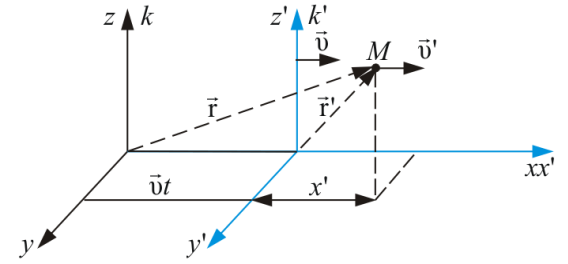
\includegraphics[width=0.7\linewidth]{imgs/q5i3.png}
\end{figure}

Найдем связь между координатами
точки M в обеих системах отсчета. Отсчет
начнем, когда начала координат систем –
совпадают, то есть $t = t'$.

Получаем так называемые преобразования Галилея:

$$\begin{cases}
    x = x' + vt \\ 
    y = y' \\
    z = z' \\
    t = t'
\end{cases}$$

В векторной форме преобразования Галилея можно записать так: $\vec{r} = \vec{r_0} + \vec{r'} = \vec{r'} + \vec{v}t$

Продифференцируем это выражение по времени, получим: закон сложения скоростей в классической механике:

$$\frac{d\vec{r}}{dt} = \frac{d\vec{r'}}{dt} + \vec{v} \implies \vec{v_1} = \vec{v'} + \vec{v}$$

Также несложно получить $\vec{a} = \vec{a_0} + \vec{a'}$ 